%----------------------------------------------------------------------------------------
%	PACKAGES AND OTHER DOCUMENT CONFIGURATIONS
%----------------------------------------------------------------------------------------

\documentclass[
11pt, % The default document font size, options: 10pt, 11pt, 12pt
a4paper,
english,
onehalfspacing, %singlespacing, % Single line spacing, alternatives: onehalfspacing or doublespacing
]{article}

%\renewcommand{\baselinestretch}{1.3}

\usepackage[T1]{fontenc}    % Output font encoding for international characters
\usepackage[utf8]{inputenc} % Required for inputting international characters

\usepackage{sectsty}

\sectionfont{\huge}
\subsectionfont{\LARGE}
\subsubsectionfont{\Large}
\paragraphfont{\large}

\setcounter{secnumdepth}{4} % Number subsubsections in the chapters
\setcounter{tocdepth}{4}    % Put paragraph in the table of contents

\usepackage{palatino} % Use the Palatino font by default
%\usepackage{courier} % Required for the courier font

\usepackage[margin=1.5in]{geometry} % Set the margins 
\usepackage{fancyhdr} % Required for custom headers
\usepackage{graphicx} % Required to insert images

\usepackage[hidelinks]{hyperref}
\usepackage{url}

\usepackage[nottoc,notlof,notlot]{tocbibind} % Include bibliography in the table of contents, remove List of Figures and Tables

\usepackage{verbatim} %for comments

%\usepackage{siunitx}

\usepackage{multicol}
\usepackage{multirow}
\usepackage{enumitem}

%\usepackage[usenames,dvipsnames]{color} % Required for custom colors
\usepackage[dvipsnames]{xcolor}
\usepackage{listings} % Required for insertion of code
\usepackage{caption}
\usepackage{framed}

\setlength{\parindent}{15pt}
\setlength{\parskip}{5pt}


%----------------------------------------------------------------------------------------
%	SET UP THE HEADER AND FOOTER
%----------------------------------------------------------------------------------------
% Set up the header and footer
\pagestyle{fancy}
\lhead{} % Top left header
\chead{} % Top center head
\rhead{\hmwkTitle} % Top right header

\lfoot{} % Bottom left footer
\cfoot{ \thepage } % Bottom center footer
\rfoot{} % Bottom right footer
\renewcommand\headrulewidth{0.4pt} % Size of the header rule
\renewcommand\footrulewidth{0.4pt} % Size of the footer rule

\newcommand{\hmwkTitle}{IPC - Inter Partition Communication} % Assignment title


\begin{document}
%----------------------------------------------------------------------------------------
%	TITLE PAGE
%----------------------------------------------------------------------------------------
\begin{titlepage}
	
	\newcommand{\HRule}{\rule{\linewidth}{0.5mm}} % Defines a new command for the horizontal lines, change thickness here
	
	\begin{center}
		% Include a department/university logo
		\begin{figure}
		\centering
		\begin{minipage}{.5\textwidth}
		  \begin{flushleft}
		  
\includegraphics[width=.4\linewidth]{Figures/EE}
		  \end{flushleft}
		\end{minipage}%
		\begin{minipage}{.5\textwidth}
		  \begin{flushright}
		  
\includegraphics[width=.4\linewidth]{Figures/CA}
		  \end{flushright}
		\end{minipage}\\[1.5cm]
		\end{figure}
		

		\textsc{\LARGE University of Minho}\\[1cm] % University name
		\textsc{\Large Embedded Systems Research Group}\\[1cm] % Thesis type
		
		\HRule \\[0.4cm] % Horizontal line
		{\huge \bfseries IPC \\ Inter Partition Communication\par}\vspace{0.4cm} % Title
		\HRule \\[2.5cm] % Horizontal line
		
%		{\scshape\Large Analysis Report\par}\vspace{1cm} % Report Type
		
%		\includegraphics[scale = 0.45]{Figures/virtualFences}\vspace{1cm}
		
		\begin{minipage}[t]{0.4\textwidth}
			\begin{flushleft} \large
				\emph{\textbf{Authors:}}\\ {José \textsc{Ribeiro} A71881 \\Nuno \textsc{Silva} A70616} 
			\end{flushleft}
		\end{minipage}
		\begin{minipage}[t]{0.4\textwidth}
			\begin{flushright} \large
				\emph{\textbf{Advisors:}} \\{Adriano \textsc{Tavares} \\Vitor \textsc{Silva}} % Supervisor name - remove the \href bracket to remove the link  
			\end{flushright}
		\end{minipage}\\[2.5cm]
		
		
%		{\large \today} % Date
		{\large Academic Year: 2016/2017}
		
		\vfill
	\end{center}
\end{titlepage}

\newpage
\pagenumbering{roman}  % Use roman page numbering style (i, ii, iii, iv...) for the pre-content pages

%----------------------------------------------------------------------------------------
%	LIST OF CONTENTS/FIGURES/TABLES PAGES
%----------------------------------------------------------------------------------------
\tableofcontents % Prints the main table of contents

\newpage
%\renewcommand{\listfigurename}{Figures}
\listoffigures % Prints the list of figures

\newpage
%\renewcommand{\listtablename}{Tables}
\listoftables % Prints the list of tables

%\newpage
%\lstlistoflistings

\newpage


%----------------------------------------------------------------------------------------
%	CONTENT - CHAPTERS/SECTIONS
%----------------------------------------------------------------------------------------

\pagenumbering{arabic} % Begin numeric (1,2,3...) page numbering

% Include the chapters of the thesis as separate files from the Chapters folder
% Uncomment the lines as you write the chapters


%----------------------------------------------------------------------------------------
%	SECTION 1
%----------------------------------------------------------------------------------------

\section{Theoretical Fundamentals}
\subsection{Waterfall Model}
The Waterfall model is a sequential model for software projects development. It is a sequential model and its name is given because of how the different phases follow one another.

\begin{figure}[!h]
	\center
	\label{figure3}
	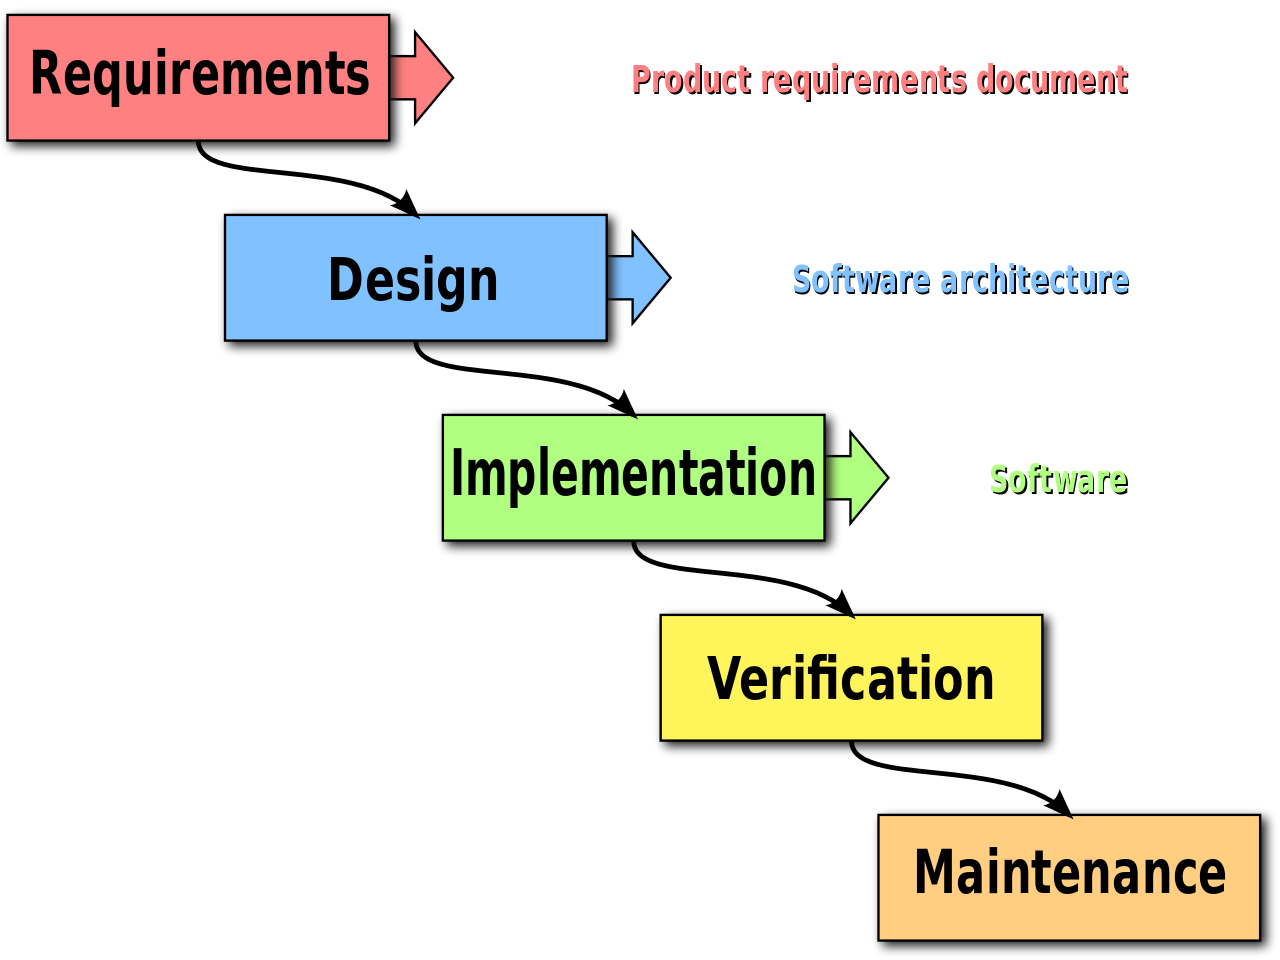
\includegraphics[scale=0.30]{Figures/waterfall} \\
	\caption {Waterfall Model}
\end{figure}

\noindent \textbf{Analysis Phase}: Execution of models and diagrams that explain the problem and its solution. It normally explains what is the problem to be solved, the requirements and constraints to solve it, as well as a brief and general hardware/software specification. It is also in this phase that a division of member’s tasks is made with also the deadlines for each different stage of the project. \\[\baselineskip]
%\newpage
\textbf{Design Phase}: A more in-depth Hardware/Software specification. In this phase, there needs to be a more scientific explanation of the problem and the solutions that will solve it.\\[\baselineskip]
\textbf{Implementation Phase}: Creation of a final prototype that solves the initial problem.\\[\baselineskip]
\textbf{Verification Phase}: Testing the final prototype in all the different situations that the product may face and do the needed changes so the final product passes those tests.\\[\baselineskip]
\textbf{Maintenance Phase}: Support and maintenance of the final product.\\[\baselineskip]
\indent In all the stages of the project a verification of the last phase should be done, before starting the following phase of the project.\\
\indent Despite being a sequential model, the Waterfall Model allows the return to earlier
phases of the project to correct mistakes that were only noticed ahead or, for example, some specification was poorly made, being possible correcting the mistakes before moving forward.

\subsection{Hypervisor}
Layer of software that allows to run several independent execution environments in a single
computer\\
\indent The bare-metal hypervisors run directly on the native hardware\\
\indent Virtualizing the critical hardware devices to create several isolated partitions

\begin{figure}[!h]
	\center
	\label{figure6}
	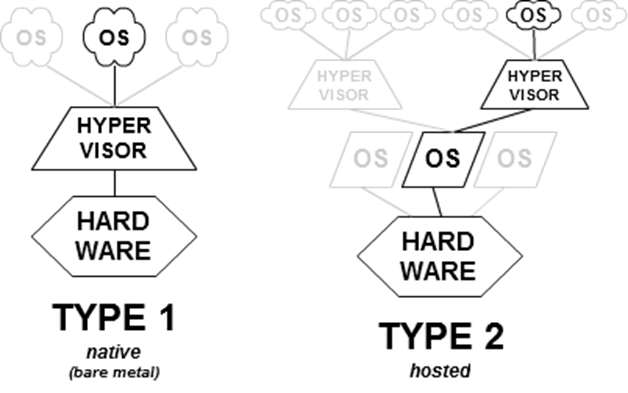
\includegraphics[scale=0.65]{Figures/Hypervisor} \\
	\caption {Hypervisor}
\end{figure}

\newpage
\section{Analysis Phase}

\subsection{Problem Statement}
In a world where the need for critical embedded systems is rising, and where also the complexity of these systems is getting bigger and bigger, there was also a need for a way to bring the best performance possible in these systems. One of these solutions was a possibility to run multiple Operating Systems in the same hardware, thus improving the performance, which was achieved with the help of an Hypervisor.\\
\indent The Hypervisor provides a layer of abstraction between the hardware and the Operating Systems, making the connection to the hardware creating a transparent feel for the OS’s. It also manages the OS’s’ scheduling times. However, when the different OS’s running on top of the Hypervisor need to communicate between each other, the regular ways of communicating, through TCP/IP or other wireless based communication protocol, are not ideal and can slow-down the performance of the system, sometimes to an unusable state.\\
\indent For that reason, a standard Hypervisor will implement an Inter-Partition Communication, or IPC, mechanism, which allows seamless communication between the different partitions through the Hypervisor layer.\\
\indent However, for some critical systems, the communication needs to be as fast as possible and one solution is to accelerate it in hardware.

\subsection{Market Study}

“Ontology-driven Metamodeling Towards Hypervisor Design Automation: Hardware based Inter-Partition Communication” by Ana Rita Fernandes Martins\\
\indent ”Shared-Memory Optimizations for Inter-Virtual-Machine Communication”\\
\indent XenLoop \cite{Nastide2010}\\

\subsection{Inter-Partition Communication (IPC)}
\begin{figure}[!htbp]
\center
\label{figure7}
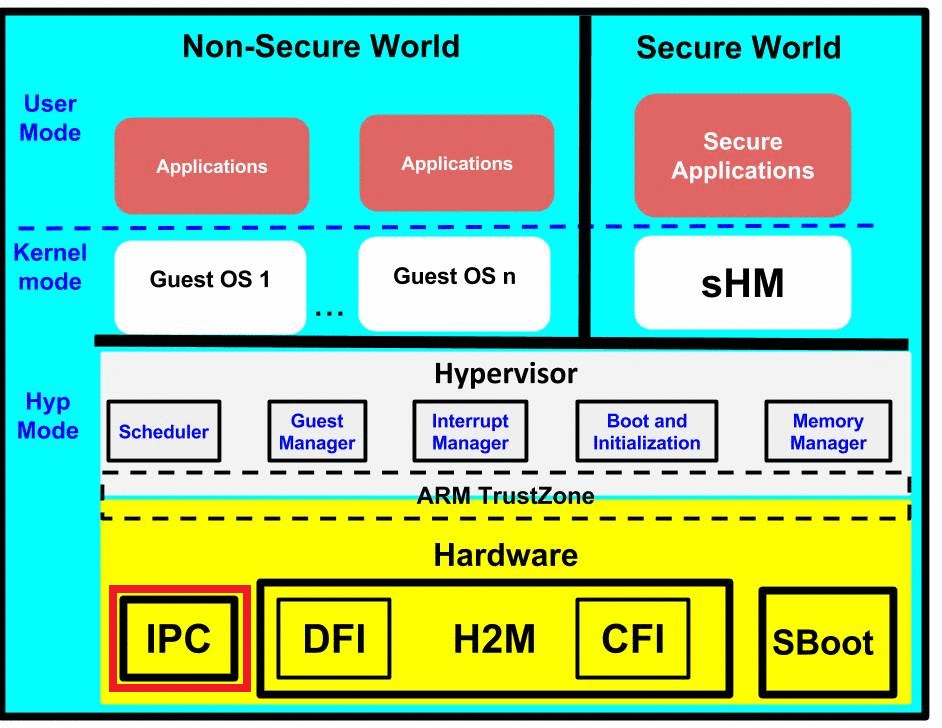
\includegraphics[scale=0.35]{Figures/IPC} \\
\caption {IPC location}
\end{figure}
To communicate between the virtualized Guest OSs there is a need for a quick communication method\\
\indent Inter-Partition Communication is a crucial module in a Hypervisor whose Guests’ need to communicate\\
\indent However, some improvements can be made by implementing the communication system directly in hardware

\subsection{Requirements}

\subsubsection{Functional Requirements}
\begin{itemize}
\item Manage communication between guest OSs
\item Accelerate the communication in hardware
\end{itemize}
\subsubsection{Non-Functional Requirements}
\begin{itemize}
\item The generated code shall be compatible with Cortex™-A9 processor architecture
\end{itemize}

\subsection{Constraints}

\subsubsection{Management}
\begin{itemize}  
	\item Meeting the specified deadlines
	\item Group composed only by two elements
	\item Limited to about 15 hours of weekly work per element
	\item The Hypervisor parts will be co-developed with other groups, making the final result depend on external factors
\end{itemize}

\subsubsection{Technical}
\begin{itemize}
	\item Use of ZYBO Zynq-7000 Development Board
	\item Integrate with \(\mu\)TZVisor
	\item Use Vivado
	\item Use Chipscope
	\item Use GNU Toolchain
\end{itemize}

\subsection{Resources}
\begin{itemize}
	\item Vivado
	\item ZYBO Zynq-7000 Development Board
\end{itemize}

\subsubsection{Use Cases}

\subsubsection{Events}

\subsubsection{State Diagram}

\subsubsection{Sequence Diagram}

\subsection{Task Division}
\begin{figure}[!htbp]
\center
\label{figure4}
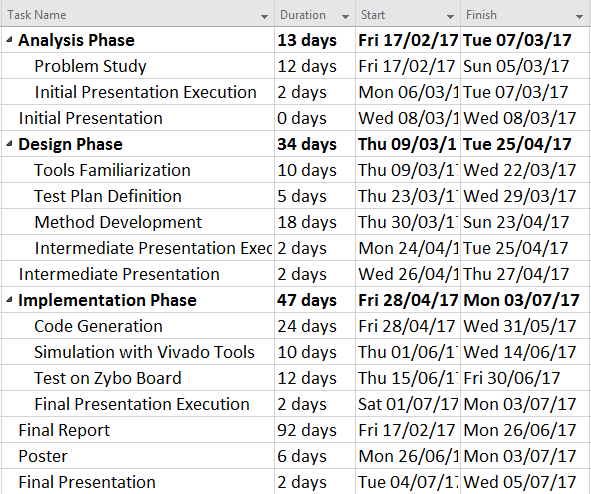
\includegraphics[scale=0.8]{Figures/TaskDivision} \\
\caption {Task Division}
\end{figure}

\subsection{Gantt Diagram}
\begin{figure}[!htbp]
\center
\label{figure5}
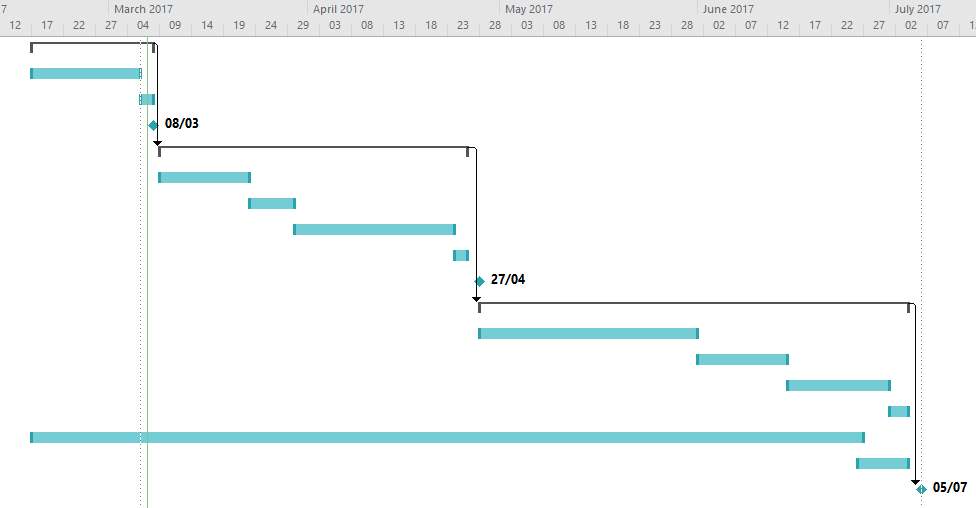
\includegraphics[scale=0.54]{Figures/Gantt} \\
\caption {Gantt Diagram}
\end{figure}
\textbf{Red:} Jose Ribeiro	\textbf{Blue:} Nuno Silva	\textbf{Green:} Both
%\FloatBarrier
\newpage


%----------------------------------------------------------------------------------------
%	SECTION 1
%----------------------------------------------------------------------------------------

\section{Design Phase}

 
%\include{Chapters/Chapter3}
%\include{Chapters/Chapter4} 
%\include{Chapters/Chapter5} 


%----------------------------------------------------------------------------------------
%	THESIS CONTENT - APPENDICES
%----------------------------------------------------------------------------------------

\appendix % Cue to tell LaTeX that the following "chapters" are Appendices

% Include the appendices of the thesis as separate files from the Appendices folder
% Uncomment the lines as you write the Appendices

%\include{Appendices/AppendixA}
%\include{Appendices/AppendixB}
%\include{Appendices/AppendixC}

%----------------------------------------------------------------------------------------
%	BIBLIOGRAPHY
%----------------------------------------------------------------------------------------

%\bibliographystyle{abbrv}
\bibliographystyle{unsrt}
\bibliography{refs}



%----------------------------------------------------------------------------------------
\end{document}